\section{Introduction}
Motor-propeller dynamics in multi-rotor vehicles are often oversimplified as
stationary mapping (\cite{tayebi2006attitude}) or reduced-order linear dynamics
(\cite{pounds2010modelling}). These models neglect the inherent polynomial
nonlinearity in actuator dynamics, including friction and aerodynamics. Previous
studies (\cite{pounds2009design},\cite{pounds2007system},\cite{mahony2012multirotor}) used rotor RPM feedback to enhance system
dynamics, relying on a second-order model around hover conditions. While
effective for minor input variations, this approach struggles with substantial
input changes. The rotational inertia and mass of large propeller blades
introduce time-scales comparable to overall drone dynamics, crucial for precise
maneuvers (\cite{hamandi2021design}).

Open-loop control, while simplifying actuator design, has limited bandwidth (Charla et al., 2022) and can amplify uncertainties. Feedback mechanisms, such as monitoring actuator inputs for aerodynamic power (\cite{B_Manony}) or propeller RPM (\cite{franchi2017adaptive}, \cite{bangura2017thrust}), are necessary but can suffer from calibration errors. Commercially available BLDC RPM sensors now enable reliable RPM measurements in medium-sized drones.

\cite{franchi2017adaptive} implemented a hybrid controller using RPM feedback to
linearize actuator dynamics, requiring low-level access to the Electronic Speed
Controller's (ESC's) microcontroller. A challenge with commercial ESCs is their
thrust-to-input curve is linearized for intuitive operability, typically
achieved by introducing nonlinear compensation in the ESC's speed controller and
the actual PWM input to the inverter controlling the BLDC motor
(Fig.~\ref{fig::bldc_diag}). This compensation is not explicitly known, making
it challenging to design a controller that can adapt to the actuator's
nonlinearities. The present work accounts for this compensation by incorporating
the static mapping between the PWM input and the steady state RPM of the
motor-propeller system into the nonlinear dynamic model.

%===
\begin{figure}[h]
    \centering
    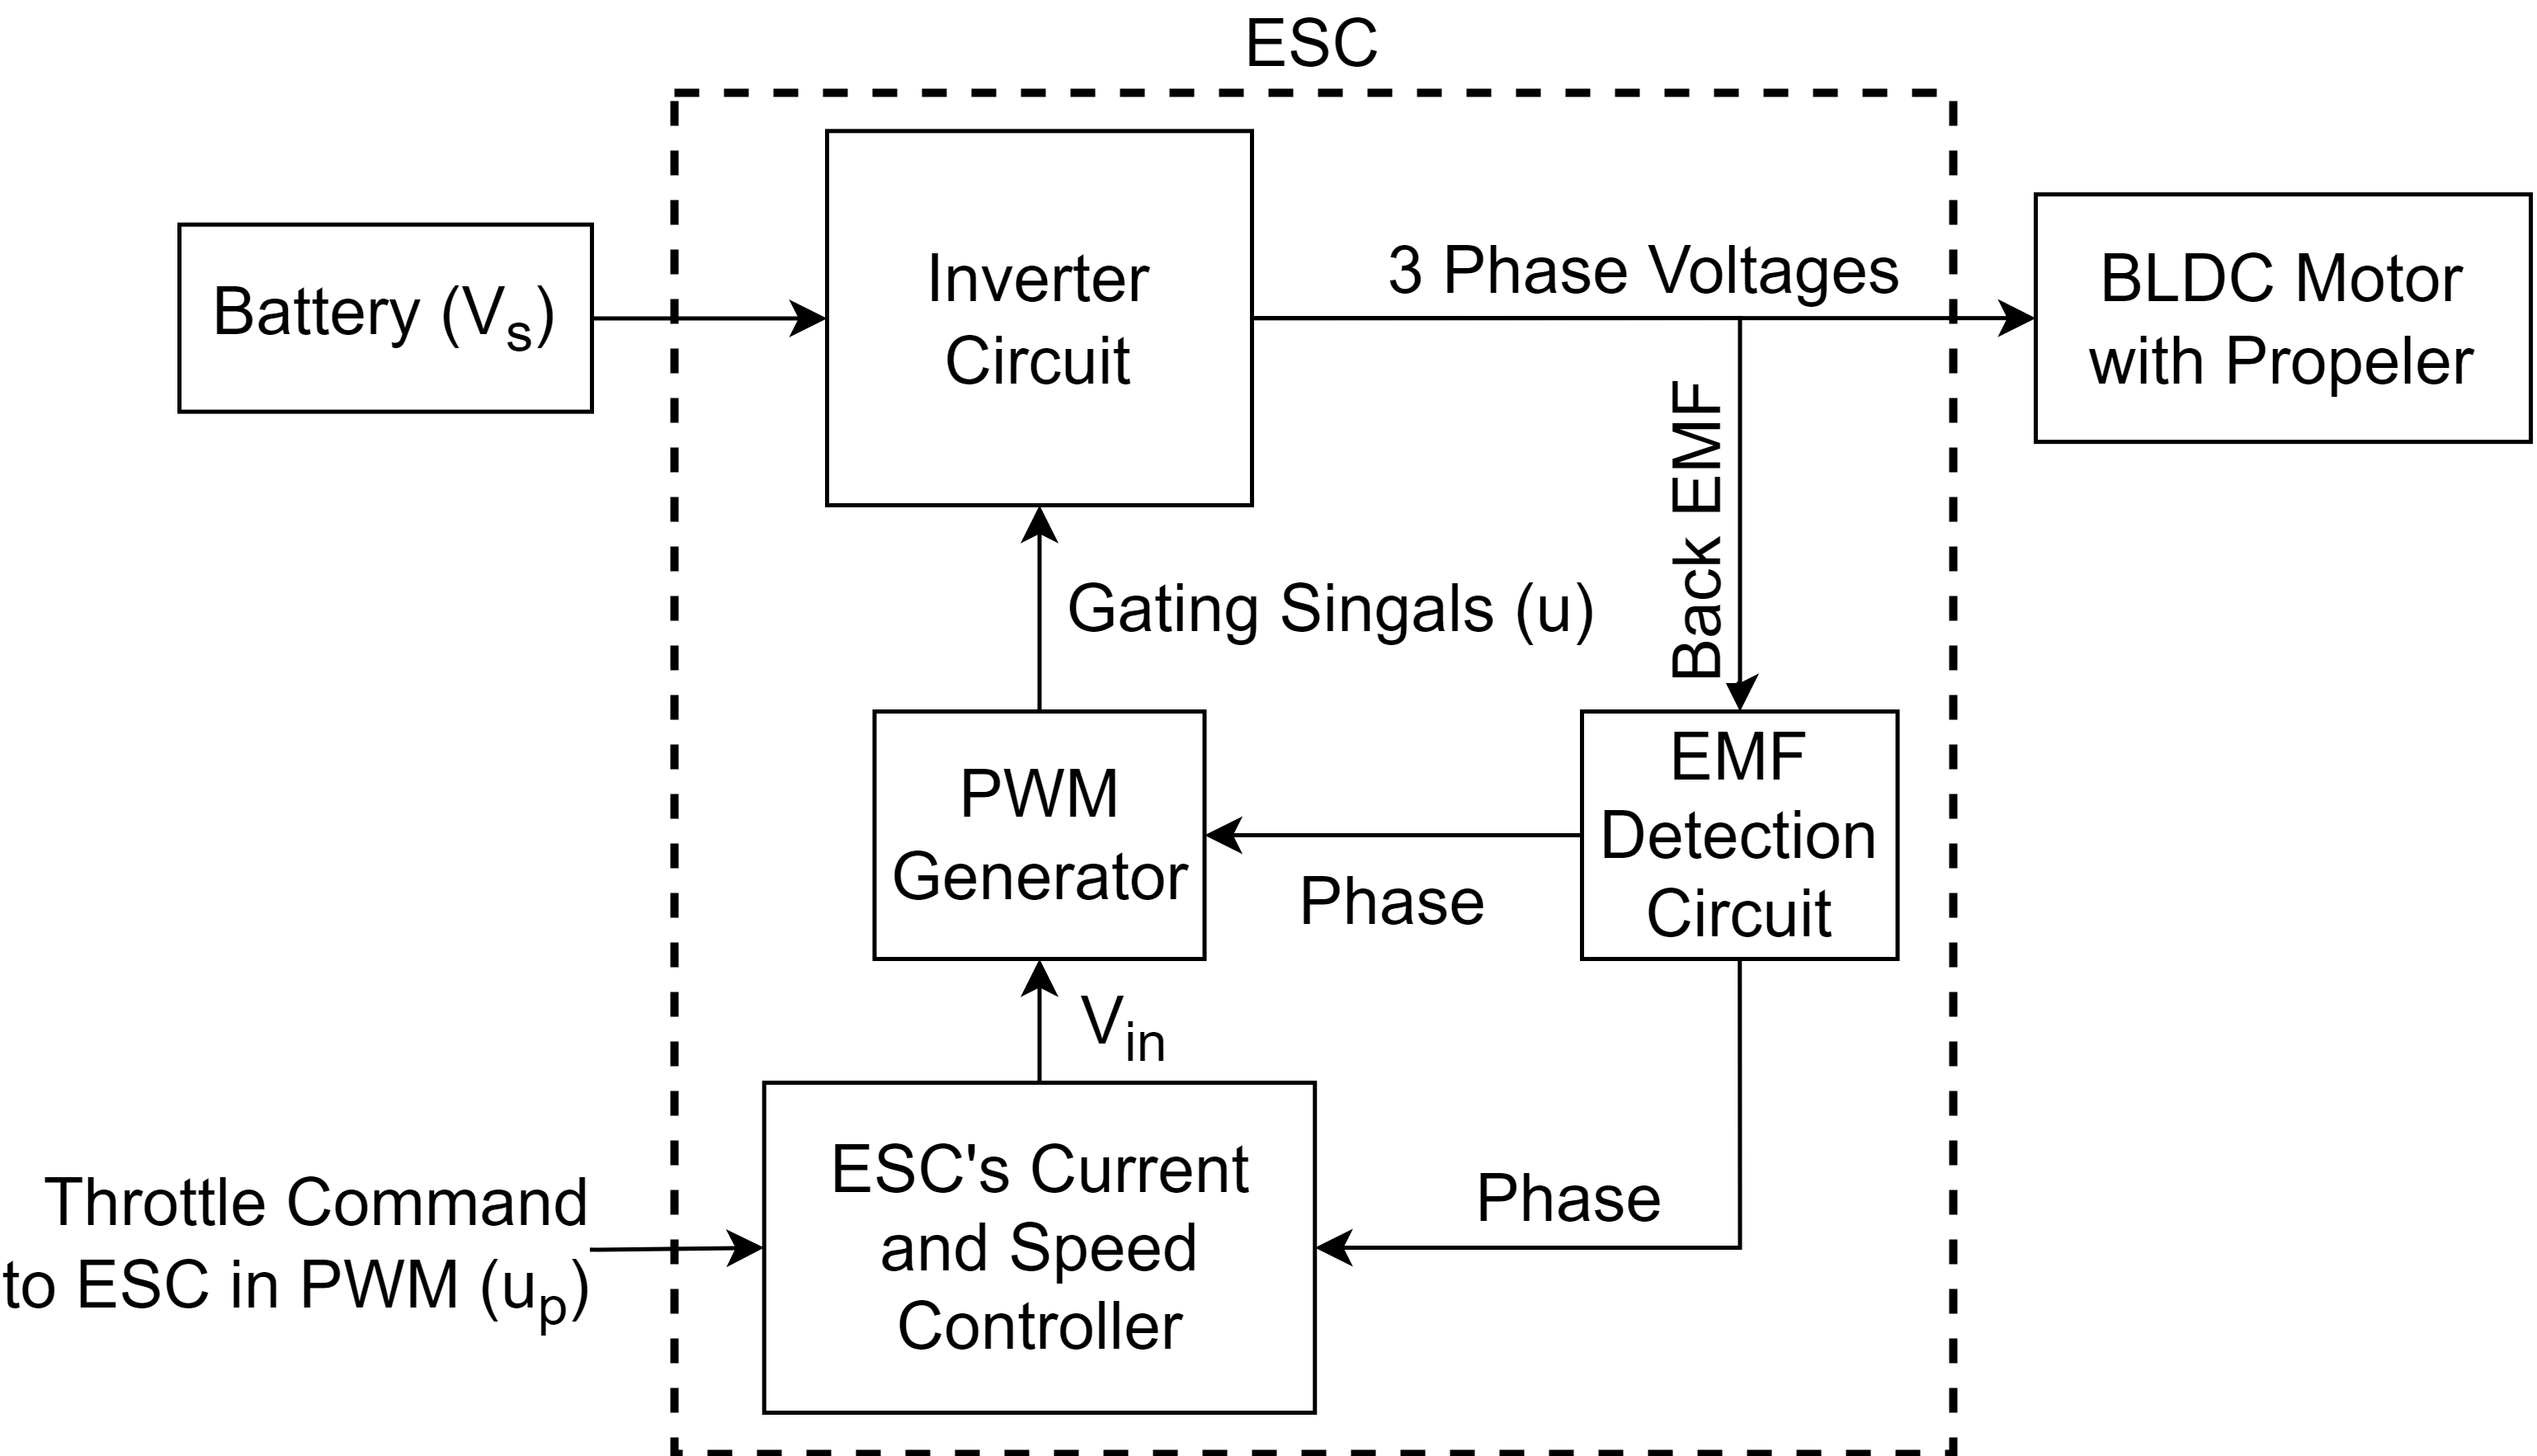
\includegraphics[width = \figsize]{./figs/figs_acc/schematic/esc_schematic.png}
    \caption{Schematic of ESC with BLDC motor}
    \label{fig::bldc_diag}
\end{figure}
%===

The motor-propeller system's function in the present context is to generate the
desired thrust $T_d$. In general this thrust is quadratic function of the
angular velocity $\omega$ of the propeller with uncertainties $(T_d = C_T
\omega_d^2 + \Delta_T)$. Let, $T (=\hat C_T \omega)$ be the thrust that has
been generated by the controller (main attitude/position control loop of the
drone) by using this thrust model and open-loop motor commands. The error in
thrust generation can be expressed as:
\begin{align*}
    e_T &= T_d - T = C_T \omega_d^2 - \hat C_T \omega^2 + 2 \Delta_T\\
        &= C_T (\omega + \omega_d) e_{\omega} + \Delta C_T \omega^2 + 2 \Delta_T
\end{align*}
Thus the thrust error $e_T$ is a function of the angular velocity error and the
uncertainties in the thrust model. Both of these errors cannot be reduced by
using attitude error feedback with limited excitation persistence. The goal of the present work is to make $e_\omega \rightarrow 0$ asymptotically
by using the RPM feedback. Such approach is expected to improve the tracking of
the thrust command ($T_d$) by reducing the thrust error ($e_T$) due to angular
velocity uncertainties and providing a linear dynamics for the actuator the can
further be used to design estimators for thrust coefficient ($C_T$)
from attitude feedback.

The proposed approach is based on a nonlinear dynamic model of the
motor-propeller system, which is identified using RPM feedback. The model is
then used to design an adaptive robust controller that can asymptotically tracks
a given reference and estimates the nonlinear model parameters in real-time. As
the RPM measurement is prone to significant noise, DCARC is used to design the
controller. The controller is then validated on a test bench.
